% \documentclass[smaller, handout
% ]{beamer}
% \usepackage{handoutWithNotes}
% \pgfpagesuselayout{2 on 1 with notes}[letterpaper, landscape, border shrink=4mm]

\def\bmode{0} % Mode 0 for presentation, mode 1 for a handout with notes, mode 2 fo% r handout without notes
\if 0\bmode
\documentclass[smaller]{beamer}
\else \if 1\bmode
\immediate\write18{pdflatex -jobname=\jobname-Handout-Notes\space\jobname}
\documentclass[smaller,handout]{beamer}
\usepackage{handoutWithNotes}
\pgfpagesuselayout{2 on 1 with notes}[letterpaper, landscape, border shrink=4mm]
\else \if 2\bmode
\immediate\write18{pdflatex -jobname=\jobname-Handout\space\jobname}
\documentclass[smaller,handout]{beamer}
\fi
\fi
\fi

%%%%%%%%%%%%%%%%%%%%%%%%%%%%%%%%%%%%%%%%%%%%%%%%%%%%%%%%%%%%%%%%%%%%%%%%%%%%%%%%%%%%%%%%%%%%%
\newcommand{\coursetitle}{CEE 616: Probabilistic Machine Learning}
\newcommand{\longlecturetitle}{Foundations: Optimization}
\newcommand{\shortlecturetitle}{1f: Optimization}
\newcommand{\instructor}{Jimi Oke}
\newcommand{\lecturedate}{Thu, Sep 18, 2025}
%%%%%%%%%%%%%%%%%%%%%%%%%%%%%%%%%%%%%%%%%%%%%%%%%%%%%%%%%%%%%%%%%%%%%%%%%%%%%%%%%%%%%%%%%%%%%


% \usepackage[T1]{fontenc} 
% \usepackage{lmodern} 
%\usepackage{etex}
 %\newcommand{\num}{6{} }

% \usetheme[
%   outer/progressbar=foot,
%   outer/numbering=fraction,
%   block=fill,
%   inner/subsectionpage=progressbar
% ]{metropolis}
\usetheme{Madrid}
\useoutertheme[subsection=false]{miniframes} % Alternatively: miniframes, infolines, split
\useinnertheme{circles}
% %\useoutertheme{Frankfurt}
% \usecolortheme{beaver}
% %\useoutertheme{crane}
% %\useoutertheme{metropolis}
\usepackage[backend=biber,style=authoryear,maxcitenames=2,maxbibnames=99,safeinputenc,url=false, eprint=false]{biblatex}
%\addbibresource{bib/references.bib}
% \AtEveryCitekey{\iffootnote{{\tiny}\tiny}{\tiny}}

% %\usepackage{pgfpages}
% %\setbeameroption{hide notes} % Only slides
% %\setbeameroption{show only notes} % Only notes
% %\setbeameroption{hide notes} % Only notes
% %\setbeameroption{show notes on second screen=right} % Both

% % \usepackage[sfdefault]{Fira Sans}

% % \setsansfont[BoldFont={Fira Sans}]{Fira Sans Light}
% % \setmonofont{Fira Mono}

% %\usepackage{fira}
% %\setsansfont{Fira}
% %\setmonofont{Fira Mono}
% % To give a presentation with the Skim reader (http://skim-app.sourceforge.net) on OSX so
% % that you see the notes on your laptop and the slides on the projector, do the following:
% % 
% % 1. Generate just the presentation (hide notes) and save to slides.pdf
% % 2. Generate onlt the notes (show only nodes) and save to notes.pdf
% % 3. With Skim open both slides.pdf and notes.pdf
% % 4. Click on slides.pdf to bring it to front.
% % 5. In Skim, under "View -> Presentation Option -> Synhcronized Noted Document"
% %    select notes.pdf.
% % 6. Now as you move around in slides.pdf the notes.pdf file will follow you.
% % 7. Arrange windows so that notes.pdf is in full screen mode on your laptop
% %    and slides.pdf is in presentation mode on the projector.

% % Give a slight yellow tint to the notes page
% \setbeamertemplate{note page}{\pagecolor{yellow!5}\insertnote}\usepackage{palatino}

% %\usetheme{metropolis}
% %\usecolortheme{beaver}
 \usepackage{tipa}
% \usepackage{enumerate}
% \definecolor{darkcandyapplered}{HTML}{A40000}
% \definecolor{lightcandyapplered}{HTML}{e74c3c}

% %\setbeamercolor{title}{fg=darkcandyapplered}

% \definecolor{UBCblue}{rgb}{0.04706, 0.13725, 0.26667} % UBC Blue (primary)
% \definecolor{UBCgrey}{rgb}{0.3686, 0.5255, 0.6235} % UBC Grey (secondary)

% % \setbeamercolor{palette primary}{bg=darkcandyapplered,fg=white}
% % \setbeamercolor{palette secondary}{bg=darkcandyapplered,fg=white}
% % \setbeamercolor{palette tertiary}{bg=darkcandyapplered,fg=white}
% % \setbeamercolor{palette quaternary}{bg=darkcandyapplered,fg=white}
% % \setbeamercolor{structure}{fg=darkcandyapplered} % itemize, enumerate, etc
% % \setbeamercolor{section in toc}{fg=darkcandyapplered} % TOC sections
% % \setbeamercolor{frametitle}{fg=darkcandyapplered,bg=white} % TOC sections
% % \setbeamercolor{title in head/foot}{bg=white,fg=white} % TOC sections
% % \setbeamercolor{button}{fg=darkcandyapplered} % TOC sections

% % % Override palette coloring with secondary
% % \setbeamercolor{subsection in head/foot}{bg=lightcandyapplered,fg=white}

%\usecolortheme{crane}
% \makeatletter
% \setbeamertemplate{headline}{%
%   \begin{beamercolorbox}[colsep=1.5pt]{upper separation line head}
%   \end{beamercolorbox}
%   \begin{beamercolorbox}{section in head/foot}
%     \vskip1pt\insertsectionnavigationhorizontal{\paperwidth}{}{}\vskip1pt
%   \end{beamercolorbox}%
%   \ifbeamer@theme@subsection%
%     \begin{beamercolorbox}[colsep=1.5pt]{middle separation line head}
%     \end{beamercolorbox}
%     \begin{beamercolorbox}[ht=2.5ex,dp=1.125ex,%
%       leftskip=.3cm,rightskip=.3cm plus1fil]{subsection in head/foot}
%       \usebeamerfont{subsection in head/foot}\insertsubsectionhead
%     \end{beamercolorbox}%
%   \fi%
%   \begin{beamercolorbox}[colsep=1.5pt]{lower separation line head}
%   \end{beamercolorbox}
% }
% \makeatother

% Reduce size of frame box
\setbeamertemplate{frametitle}{%
    \nointerlineskip%
    \begin{beamercolorbox}[wd=\paperwidth,ht=2.0ex,dp=0.6ex]{frametitle}
        \hspace*{1ex}\insertframetitle%
    \end{beamercolorbox}%
}


%\setbeamercolor{frametitle}{bg=darkcandyapplered!80!black!90!white}
%\setbeamertemplate{frametitle}{\bf\insertframetitle}

%\setbeamercolor{footnote mark}{fg=darkcandyapplered}
%\setbeamercolor{footnote}{fg=darkcandyapplered!70}
%\Raggedbottom
%\setbeamerfont{page number in head/foot}{size=\tiny}
%\usepackage[tracking]{microtype}


% %\usepackage[sc,osf]{mathpazo}   % With old-style figures and real smallcaps.
% %\linespread{1.025}              % Palatino leads a little more leading

% % Euler for math and numbers
% %\usepackage[euler-digits,small]{eulervm}
% %\AtBeginDocument{\renewcommand{\hbar}{\hslash}}
\usepackage{graphicx,multirow,booktabs}
\usepackage{animate}
\usepackage{media9}


% %\mode<presentation> { \setbeamercovered{transparent} }

\setbeamertemplate{navigation symbols}{}
\makeatletter
\def\beamerorig@set@color{%
  \pdfliteral{\current@color}%
  \aftergroup\reset@color
}
\def\beamerorig@reset@color{\pdfliteral{\current@color}}
\makeatother


% %=== GRAPHICS PATH ===========
\graphicspath{{./images/}}
% % Marginpar width
% %Marginpar width
% %\setlength{\marginparsep}{.02in}


% %% Captions
% % \usepackage{caption}
% % \captionsetup{
% %   labelsep=quad,
% %   justification=raggedright,
% %   labelfont=sc
% % }

% \setbeamerfont{caption}{size=\footnotesize}
% \setbeamercolor{caption name}{fg=darkcandyapplered}

% %AMS-TeX packages

\usepackage{amssymb,amsmath,amsthm,mathtools} 
\usepackage{bm}
\DeclareMathOperator*{\argmax}{arg\,max}
\DeclareMathOperator*{\argmin}{arg\,min}
% \usepackage{color}

% %https://tex.stackexchange.com/a/31370/2269
% \usepackage{mathtools,cancel}

% \renewcommand{\CancelColor}{\color{red}} %change cancel color to red

% \makeatletter
% \let\my@cancelto\cancelto %copy over the original cancelto command
% \newcommand<>{\cancelto}[2]{\alt#3{\my@cancelto{#1}{#2}}{\mathrlap{#2}\phantom{\my@cancelto{#1}{#2}}}}
% % redefine the cancelto command, using \phantom to assure that the
% % result doesn't wiggle up and down with and without the arrow
% \makeatother


% %\usepackage{comment}
% %\usepackage{hyperref,enumerate}
% \usepackage{minitoc,array}

% \definecolor{slblue}{rgb}{0,.3,.62}
% % \hypersetup{
% %     colorlinks,%
% %     citecolor=blue,%
% %     filecolor=blue,%
% %     linkcolor=blue,
% %     urlcolor=slblue
% % }

% \usepackage{epstopdf}
% \epstopdfDeclareGraphicsRule{.gif}{png}{.png}{convert gif:#1 png:\OutputFile}
% \AppendGraphicsExtensions{.gif}

% %\usepackage{listings}

% %%% TIKZ
% \usepackage{forest}
\usepackage{tikz}
\usepackage{pgfplots}
\usepackage{pgfplotstable}
%\usepackage{pgfgantt}
\pgfplotsset{compat=newest}

\usetikzlibrary{fit,arrows,shapes,positioning,shapes.geometric}
\usetikzlibrary{decorations.markings}
\usetikzlibrary{shadows,automata}
\usetikzlibrary{patterns}
\usetikzlibrary{trees,mindmap,backgrounds}
%\usetikzlibrary{circuits.ee.IEC}
\usetikzlibrary{decorations.text}
% % For Sagnac Picture
% \usetikzlibrary{%
%     decorations.pathreplacing,%
%     decorations.pathmorphing%
% }
% \tikzset{no shadows/.style={general shadow/.style=}}
% %
% %\usepackage{paralist}

% \tikzset{
%   font=\Large\sffamily\bfseries,
%   red arrow/.style={
%     midway,red,sloped,fill, minimum height=3cm, single arrow, single arrow head extend=.5cm, single arrow head indent=.25cm,xscale=0.3,yscale=0.15,
%     allow upside down
%   },
%   black arrow/.style 2 args={-stealth, shorten >=#1, shorten <=#2},
%   black arrow/.default={1mm}{1mm},
%   tree box/.style={draw, rounded corners, inner sep=1em},
%   node box/.style={white, draw=black, text=black, rectangle, rounded corners},
% }

% %%% FORMAT PYTHON CODE
% %\usepackage{listings}
% % Default fixed font does not support bold face
% \DeclareFixedFont{\ttb}{T1}{txtt}{bx}{n}{8} % for bold
% \DeclareFixedFont{\ttm}{T1}{txtt}{m}{n}{8}  % for normal

% % Custom colors
% \definecolor{deepblue}{rgb}{0,0,0.5}
% \definecolor{deepred}{rgb}{0.6,0,0}
% \definecolor{deepgreen}{rgb}{0,0.5,0}

% %\usepackage{animate}

% % Python style for highlighting
% % \newcommand\pythonstyle{\lstset{
% % language=Python,
% % basicstyle=\footnotesize\ttm,
% % otherkeywords={self},             % Add keywords here
% % keywordstyle=\footnotesize\ttb\color{deepblue},
% % emph={MyClass,__init__},          % Custom highlighting
% % emphstyle=\footnotesize\ttb\color{deepred},    % Custom highlighting style
% % stringstyle=\color{deepgreen},
% % frame=tb,                         % Any extra options here
%     % showstringspaces=false            % 
% % }}

% % % Python environment
% % \lstnewenvironment{python}[1][]
% % {
% % \pythonstyle
% % \lstset{#1}
% % }
% % {}

% % % Python for external files
% % \newcommand\pythonexternal[2][]{{
% % \pythonstyle
% % \lstinputlisting[#1]{#2}}}

% % Python for inline
% % 
% % \newcommand\pythoninline[1]{{\pythonstyle\lstinline!#1!}}

% %\usepackage{algorithm2e}

\newcommand{\eps}{\epsilon}
\newcommand{\bX}{\mb X}
\newcommand{\by}{\mb y}
\newcommand{\bbe}{\bm\beta}
\newcommand{\beps}{\bm\epsilon}
\newcommand{\bY}{\mb Y}

\newcommand{\osn}{\oldstylenums}
\newcommand{\dg}{^{\circ}}
\newcommand{\lt}{\left}
\newcommand{\rt}{\right}
\newcommand{\pt}{\phantom}
\newcommand{\tf}{\therefore}
\newcommand{\?}{\stackrel{?}{=}}
\newcommand{\fr}{\frac}
\newcommand{\dfr}{\dfrac}
\newcommand{\ul}{\underline}
\newcommand{\tn}{\tabularnewline}
\newcommand{\nl}{\newline}
\newcommand\relph[1]{\mathrel{\phantom{#1}}}
\newcommand{\cm}{\checkmark}
\newcommand{\ol}{\overline}
\newcommand{\rd}{\color{red}}
\newcommand{\bl}{\color{blue}}
\newcommand{\pl}{\color{purple}}
\newcommand{\og}{\color{orange!90!black}}
\newcommand{\gr}{\color{green!40!black}}
\newcommand{\dca}{\color{darkcandyapplered}}
\newcommand{\nin}{\noindent}
\newcommand*\circled[1]{\tikz[baseline=(char.base)]{
            \node[shape=circle,draw,thick,inner sep=1pt] (char) {\small #1};}}

\newcommand{\bc}{\begin{compactenum}[\quad--]}
\newcommand{\ec}{\end{compactenum}}

\newcommand{\p}{\partial}
\newcommand{\pd}[2]{\frac{\partial{#1}}{\partial{#2}}}
\newcommand{\dpd}[2]{\dfrac{\partial{#1}}{\partial{#2}}}
\newcommand{\pdd}[2]{\frac{\partial^2{#1}}{\partial{#2}^2}}
\newcommand{\pde}[3]{\frac{\partial^2{#1}}{\partial{#2}\partial{#3}}}
\newcommand{\nmfr}[3]{\Phi\left(\frac{{#1} - {#2}}{#3}\right)}
\newcommand{\Err}{\text{Err}}
\newcommand{\err}{\text{err}}

%\DeclarePairedDelimiter\ceil{\lceil}{\rceil}
%\DeclarePairedDelimiter\floor{\lfloor}{\rfloor}

%%%% GREEK LETTER SHORTCUTS %%%%%
\newcommand{\la}{\lambda}
\renewcommand{\th}{\theta}
\newcommand{\al}{\alpha}
\newcommand{\G}{\Gamma}
\newcommand{\si}{\sigma}
\newcommand{\Si}{\Sigma}


\pgfmathdeclarefunction{poiss}{1}{%
  \pgfmathparse{(#1^x)*exp(-#1)/(x!)}%
  }

\pgfmathdeclarefunction{gauss}{2}{%
  \pgfmathparse{1/(#2*sqrt(2*pi))*exp(-((x-#1)^2)/(2*#2^2))}%
}

\pgfmathdeclarefunction{expo}{2}{%
  \pgfmathparse{#1*exp(-#1*#2)}%
}

\pgfmathdeclarefunction{expocdf}{2}{%
  \pgfmathparse{1 -exp(-#1*#2)}%
}

\newcommand{\mb}{\mathbb}
\newcommand{\mc}{\mathcal}
\newcommand{\tr}{^{\top}}
\newcommand{\pe}{\pause}
% \usepackage{pst-plot}

% \usepackage{pstricks-add}
% \usepackage{auto-pst-pdf}   

% \psset{unit = 3}

% \def\target(#1,#2){%
%  {\psset{fillstyle = solid}
%   \rput(#1,#2){%
%     \pscircle[fillcolor = white](0.7,0.7){0.7}
%     \pscircle[fillcolor = blue!60](0.7,0.7){0.5}
%     \pscircle[fillcolor = white](0.7,0.7){0.3}
%     \pscircle[fillcolor = red!80](0.7,0.7){0.1}}}}
% \def\dots[#1](#2,#3){%
%     \psRandom[
%       dotsize = 2pt,
%       randomPoints = 25
%     ](!#2 #1 0.04 sub sub #3 #1 0.04 sub sub)%
%      (!#2 #1 0.04 sub add #3 #1 0.04 sub add)%
%      {\pscircle[linestyle = none](#2,#3){#1}}}


%%%%%%%%%%%%%%%%%%%%%%%%%%%%%%%%%%%%%%%%%%%%%%%%%%%
%%%%%%%%%%%%%%%%%%%%%%%%%%%%%%%%%%%%%%%%%%%%%%%%%%%
\title[\shortlecturetitle]{ {\normalsize \coursetitle}
  \\ \longlecturetitle}
\date[\lecturedate]{\footnotesize \lecturedate}
\author{{\bf \instructor}}
\institute[UMass Amherst]{
%\titlegraphic{\hfill
  \begin{tikzpicture}[baseline=(current bounding box.center)]
    \node[anchor=base] at (-7,0) (its) {
\includegraphics[scale=.3]{UMassEngineering_vert}} ;
  \end{tikzpicture}
  % \hfill\includegraphics[height=1.5cm]{logo}
}

%https://tex.stackexchange.com/questions/55806/mindmap-tikzpicture-in-beamer-reveal-step-by-step
  \tikzset{
    invisible/.style={opacity=0},
    visible on/.style={alt={#1{}{invisible}}},
    alt/.code args={<#1>#2#3}{%
      \alt<#1>{\pgfkeysalso{#2}}{\pgfkeysalso{#3}} % \pgfkeysalso doesn't change the path
    },
  }


% https://tex.stackexchange.com/questions/446468/labels-with-arrows-for-an-equation
% https://tex.stackexchange.com/a/402466/121799
\newcommand{\tikzmark}[3][]{
\ifmmode
\tikz[remember picture,baseline=(#2.base)] \node [inner sep=0pt,#1](#2) {$#3$};
\else
\tikz[remember picture,baseline=(#2.base)] \node [inner sep=0pt,#1](#2) {#3};
\fi
}

% \lstset{language=matlab,
%                 basicstyle=\scriptsize\ttfamily,
%                 keywordstyle=\color{blue}\ttfamily,
%                 stringstyle=\color{blue}\ttfamily,
%                 commentstyle=\color{gray}\ttfamily,
%                 morecomment=[l][\color{gray}]{\#}
%               }


              
\begin{document}

\maketitle

\begin{frame}
  \frametitle{Outline}
  \tableofcontents
\end{frame}

\section{Inroduction}



  \begin{frame}
  \frametitle{Optimization}\pause
  Optimization is the body of mathematics that deals with the theory and algorithms for characterizing the maximum/minimum values of functions.\pause

  \begin{center}
    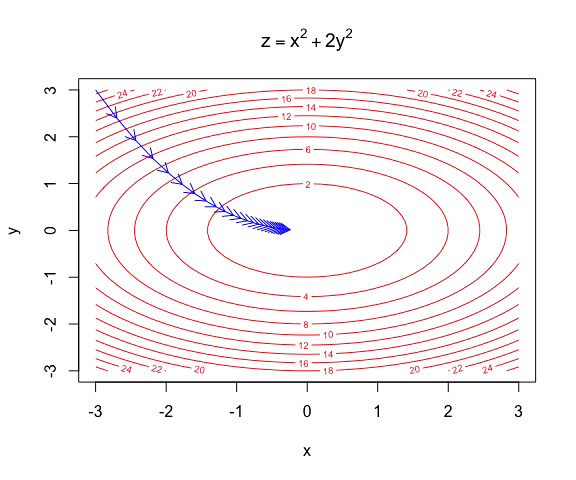
\includegraphics[width=.5\textwidth]{opt-demo}
  \end{center}

  \pause

  We will consider two widely-used approaches in machine learning:\pause

  \begin{itemize}[<+->]
  \item First-order methods (e.g.\ gradient descent)
  \item Second-order methods (e.g.\ Newton's method)
  \end{itemize}
\end{frame}

\begin{frame}
  \frametitle{Definitions} \pause

  \begin{itemize}[<+->]
    \item Minimum of convex function \pause
  \begin{equation}
    \th^{*} = \pause \arg\min_{\th} \mc{L}(\th): \pause \fr{d \mc{L}(\th^{*})}{d\th} = 0
  \end{equation}

  \pause
  
  \item Derivative of a function: \pause
    \begin{equation}
      \mc{L}'(\th) = \pause \fr{d \mc{L}(\th)}{d\th}
    \end{equation}
    \pause
  \item Gradient of a function \pause (vector of partial derivatives): \pause
    \begin{equation}
      \nabla_{\bm\th} \mc{L}(\bm \th) = \pause
      \begin{bmatrix}
        \pd{\mc{L}(\bm \th)}{\th_{1}} \\ \pause
        \pd{\mc{L}(\bm \th)}{\th_{2}} \\\pause
        \vdots \\\pause
        \pd{\mc{L}(\bm \th)}{\th_{n}} \\        
      \end{bmatrix}
    \end{equation}
     \end{itemize}

\end{frame}

\begin{frame}
  \frametitle{Further definitions}
  \pause
  \begin{itemize}
  \item Second-order derivative: \pause
    \begin{equation}
      \mc{L}''(\th) = \pause \fr{d^{2}\mc{L}(\th)}{d\th^{2}}
    \end{equation}
    
    \bigskip\pause
  \item Hessian (matrix of partial second derivatives):\pause
    \begin{equation}
      \bm H_{\bm\th}(\mc{L}(\bm\th)) = \nabla^{2}_{\bm\th}\mc{L}(\th) \pause =
      \begin{bmatrix}
        \pdd{\mc{L}(\bm \th)}{\th_{1}} & \pde{\mc{L}(\bm \th)}{\th_{1}}{\th_{2}} & \cdots & \pde{\mc{L}(\bm \th)}{\th_{1}}{\th_{n}} \\[2mm]
        \pde{\mc{L}(\bm \th)}{\th_{2}}{\th_{1}} & \pdd{\mc{L}(\bm \th)}{\th_{2}} &  \cdots & \pde{\mc{L}(\bm \th)}{\th_{2}}{\th_{n}} \\[2mm]
        \vdots & \vdots & \ddots & \vdots \\[2mm]
        \pde{\mc{L}(\bm \th)}{\th_{n}}{\th_{1}} & \pde{\mc{L}(\bm \th)}{\th_{n}}{\th_{2}}&  \cdots & \pdd{\mc{L}(\bm \th)}{\th_{n}} \\[2mm]
      \end{bmatrix}      
    \end{equation}

    \pause


  \end{itemize}
 
\end{frame}

\begin{frame}
  \frametitle{Optimality conditions}
  \pe
  For continuous, twice-differentiable functions:\pe
  \begin{itemize}
  \item If $\bm\th^*$ is a local minimum, then $\bm g^* = \bm 0$ and $\bm H^*$ must be psd (necessary condition) \pe

    \item If $\bm g^* = \bm 0$ and $\bm H^*$ is pd, then $\bm\th^*$ is a local optimum (suficient condition)
    \end{itemize}

    \pe
    \begin{block}{General approach}
      \pe
      \begin{itemize}
      \item Begin with an initial value $\bm\th_{0}$\pe
      \item At each iteration $t$, update $\bm\th_{t+1}$
      \item Terminate when $\mc{L}(\bm\th_{t+1})- \mc{L}(\bm\th_{t}) = \epsilon$
      \end{itemize}
    \end{block}
\end{frame}

\begin{frame}
  \frametitle{Convex optimization}
  \pe
  If the objective is convex and defined over a convex set, then every local minimum is a global minimum.
  pe
  \begin{itemize}
  \item Convex set: For any $\bm x$, $\bm x' \in \mc{S}$: \pe
    \begin{equation}
      \la \bm x + (1-\la)\bm x' \in \mc{S}, \quad \forall\la \in [0,1]
    \end{equation}
    \pe
  \item Convex function: For any $\bm x, \bm y \in \mc{S}$ and for any $0\le\la\le1$:\pe
    \begin{equation}
      f(\la\bm x + (1-\la)\bm y) \le \la f(\bm x) + (1-\la)f(\bm y)
    \end{equation}
  \end{itemize}
  \pe
  \begin{block}{Quadratic form}
    Given $f(\bm x)= \bm x\tr \bm A\bm x$:\pe
    \begin{itemize}
    \item $f$ is convex if $\bm A$ is psd
    \item $f$ is strictly convex if $\bm A$ is pd
    \end{itemize}
  \end{block}
\end{frame}

\begin{frame}
  \frametitle{Subgradients}
  \pe Given a convex function $f:\mb{R}^{n}\to \mb{R}$, $\bm g\in \mb{R}^{n}$ is a subgradient of $f$ at
  $\bm x \in \text{dom}(f)$ if:\pe
  \begin{equation}
    f(\bm z) \ge f(\bm x) + \bm g\tr(\bm z- \bm x)\quad \forall \bm z\in \text{dom}(f)
  \end{equation}
  \pe
  \begin{itemize}
  \item The set of subgradients is called the \textbf{subdifferential}: $\partial f(\bm x)$\pe
  \item   $f$ is subdifferentiable at $\bm x$ if it has at least one subgradient at that point
  \end{itemize}
  \pe
  \begin{exampleblock}{Subdifferential of ReLU}\pe
    The rectified linear unit function (ReLU) is given by:\pe
    \begin{equation}
      \text{ReLU}(z) = \max(0,z),\quad z\in\mb R
    \end{equation}\pe
    Its subdifferential is: \pe
    \begin{equation}
      \partial\text{ReLU}(z) =
      \begin{cases}
        0 & \text{if } z < 0 \\
        [0,1] & \text{if } z = 0 \\
        1 & \text{if } z > 0 
      \end{cases}
    \end{equation}
  \end{exampleblock}
\end{frame}

\section{First-order methods}

\begin{frame}
  \frametitle{First-order methods}
  \pause

  These methods only require first-order derivatives in order to compute an update: \pause
  \begin{equation}
    \bm\th_{t+1} = \bm\th_{t} + \rho_{t}\bm d_{t}
  \end{equation}
  \pause
  where:\pause
  \begin{itemize}
  \item $\rho_{t}$: step size/learning rate \pe
  \item $\bm d_{t}$: descent direction (e.g. negative gradient)\pe
  \item $t$: index of iteration
  \end{itemize}
  \pe
  The classic first-order method is \textbf{gradient descent}

\end{frame}


\begin{frame}
  \frametitle{Descent direction}
  \pe
  A vector $\bm d$ is considered a descent direction if a nonzero step size $\rho$ moved in its direction  yields a decrease in the objective: \pe
  \begin{equation}
    \mc{L}(\bm\th +\rho\bm d) < \mc{L}(\bm\th) \quad \forall 0 < \rho <\rho_{\max}
  \end{equation}

  \pause
  \begin{block}{Steepest descent}
    \pe
    The direction of steepest descent is given by the negative gradient: \pe
    \begin{equation}
      -\bm g_{t} = -\nabla\mc{L}(\bm\th_{t})
    \end{equation}
    \pause
    
  \end{block}
\end{frame}

\begin{frame}
  \frametitle{Step size}
  \pe The choice of step size impacts the convergence of an optimization routine. It determines how far along in the
  descent direction the variable is updated at each step.
  \pause
  \begin{itemize}
  \item \textbf{Constant step size}: $\rho$ is fixed throughout\pe
  \item \textbf{Adaptive step size}: $\rho_{t}$ is modified at each iteration to satisfy certain conditions (e.g.\ line search methods)\pe
\item Sequence $\{\rho_{t}\}$ in an optimization algorithm is known as the learning rate schedule
  \end{itemize}
\end{frame}

\begin{frame}
  \frametitle{Example: Gradient descent }\pause
  Given the function \pause
  \begin{equation*}
    \bl f(x) = (x-1)^4 - 3x + 4
  \end{equation*}
  \pause
  find the optimal point $(x^*, f(x^*))$.\pause

  \bigskip

  First, we find the \textbf{\rd gradient} and define the \textbf{\gr update} step:\pause
  \begin{eqnarray*}
    \rd f'(x) &=& \rd \pause 4(x-1)^3 - 3 \\ \pause
    \gr x_{k+1} &=&\gr \pause x_k - \lambda \lt[4(x_k -1)^3 - 3  \rt] 
  \end{eqnarray*}

  We choose $\lambda = 0.05$ and a random starting point between 0 and 1.
\end{frame}

\begin{frame}
  \frametitle{Example: Gradient descent  (cont.)}
  \pause
  \begin{center}
    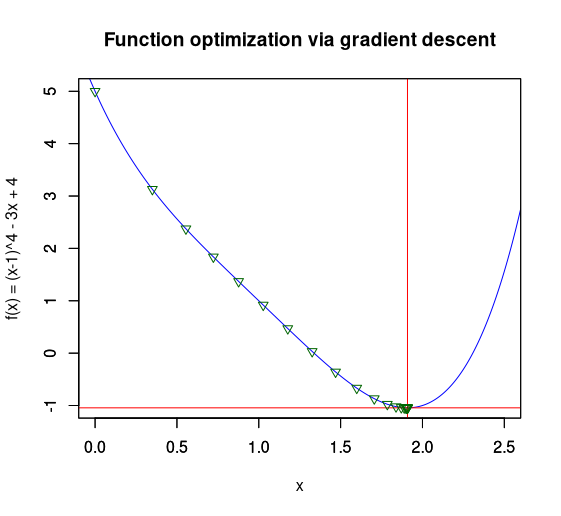
\includegraphics[width=.5\textwidth]{grad-des}
  \end{center}
  Using the \texttt{gradient-descent.ipynb} notebook, we find the optimal point as $\gr\bm{(1.908,-1.044)}$. \pause
  {\rd How does the learning rate impact the solution process?}
\end{frame}


\begin{frame}
  \frametitle{Exact line search}
  \pe
  Finds optimal  $\rho_{t}$ by:\pe
    \begin{equation}
      \rho_{t}^{*} = \pause \argmin_{\rho>0} \phi_{t}(\rho)  \pe =  \argmin_{\rho>0} \mc{L}(\bm\th_{t} + \rho\bm d_{t})
    \end{equation}
    \pe
    If $\mc{L}(\bm\th)$ is quadratic, then we can write:\pe
    \begin{equation}
      \phi_{t}(\rho) \pe= \mc{L}(\bm\th_{t} + \rho\bm d_{t}) \pe= \fr12(\bm\th + \rho\bm d)\tr\bm A(\bm\th + \rho\bm d) + \bm b\tr(\bm\th + \rho\bm d) + c
    \end{equation}
    \pe
    Solving for $\phi_{t}'(\rho) = 0$ gives the optimal update as: \pe
    \begin{equation}
      \rho_{t}^{*} = -\fr{\bm d\tr (\bm A\bm\th_{t} + \bm b)}{\bm d_{t}\tr\bm A\bm d_{t}}
    \end{equation}
    \pe
    This approach introduces additional computational expense
  \end{frame}

  \begin{frame}
    \frametitle{Armijo backtracking}
    Finds a suitable $\rho_{t}^{*}$ by iteratively shrinking $\rho_{t}$ by $\beta \in (0,1)$, i.e.\pe
    \begin{equation}
      \rho_{t}^{k+1} = \beta\rho_{t}^{k}
    \end{equation}
    until the \textbf{Armijo-Goldstein} condition is satisfied: \pe
    \begin{equation}
      \mc{L}(\bm\th_{t} + \rho\bm d_{t}) \le \mc{L}(\bm\th_{t}) + c\rho\bm d_{t}\tr\nabla\mc{L}(\bm\th_{t})
    \end{equation}
    \pe
    where $c \in [0,1]$ is typically chosen as $10^{-4}$
\end{frame}

\begin{frame}
  \frametitle{Momentum}
  \pe
  Momentum methods are used to improve convergence. \pe The momentum update is given by:\pe
  \begin{equation}
    \bm m_{t+1} = \pe \beta\bm m_{t} + \bm g_{t}
  \end{equation}
  \pe where $\beta \in (0,1)$. \pe

 
  The momentum can also be expressed as an exponentially weighted average of past gradients:  \pe
  \begin{equation}
    \bm m_{t+1} = \sum_{\tau = 0}^{t}\beta^\tau\bm g_{t-\tau}
  \end{equation}
  \pe

   The update is given by:\pe
  \begin{equation}
    \bm\th_{t+1} = \bm\th_{t} - \rho_{t}\bm m_{t+1}
  \end{equation}
 
\end{frame}

\begin{frame}
  \frametitle{Nesterov momentum}
  \pe
  In the Nesterov method, the momentum update computes the gradient at the new location, which can speed up convergence:
  \begin{equation}
    \bm m_{t+1} = \pe \beta\bm m_{t} - \rho_t\nabla\mc{L}(\bm\th_t+\beta \bm m_{t})
  \end{equation}
  \pe

  The update is given by: \pe
  \begin{equation}
    \bm\th_{t+1} \pe = \bm\th_t+\bm m_{t+1}
  \end{equation}
  \pe
  This method is also called \textbf{Nesterov accelerated gradient}
\end{frame}

\begin{frame}
  \frametitle{Stochastic gradient descent (SGD)}
  In stochastic optimization, goal is to minimize:\pe
  \begin{equation}
    \mc{L}(\bm\th) = \mb{E}_{q(\bm z)}[\mc{L}(\bm\th,\bm z)]
  \end{equation}
  \pe
  where $\bm z_t \sim q$ could be a training sample drawn from a set. \pe Thus, the \textbf{stochastic gradient descent} update is given by:\pe
  \begin{equation}
    \bm\th_{t+1} = \bm_t -\rho_t\nabla\mc{L}(\bm\th_t,\bm z_t) = \pe \bm\th_t - \rho_t\bm g_t
  \end{equation}
  \pe
  \begin{itemize}
  \item Finite sum: $\mc{L}(\bm\th_t) = \fr1N\sum_{n=1}^N\mc{L}_n(\bm\th_t)$
  \end{itemize}
\end{frame}

\section{Second-order methods}
\begin{frame}
  \frametitle{Newton's method}
  \pe Second-order methods incorporate curvature via the second derivative to speed up convergence. \pe

  The basic method of this form is Newton's method:\pe
  \begin{equation}
    \bm\th_{t+1}  \pe = \bm\th_t - \rho_t\bm{H}^{-1}\bm g_t
  \end{equation}
  \pe
  where:
  \pe
  \begin{equation}
    \bm H_t := \nabla^2\mc{L}(\bm\th_t) \pe = \bm H(\bm\th_t)
  \end{equation}
  
\end{frame}

\begin{frame}
  \frametitle{Derivation of Newton's method}
  \pe
  Taylor-expand $\mc{L}(\bm\th)$ around $\bm\th_t$:\pe
  \begin{equation}
    \mc{L}_{\text{quad}} = \mc{L}(\bm\th_t) + \bm g_t\tr(\bm\th - \bm\th_t) + \fr12(\bm\th - \bm\th_t)\tr\bm H_t(\bm\th - \bm\th_t)
  \end{equation}
  \pe
  Taking the derivative of $\mc{L}_{\text{quad}}$ and setting it to zero to find the minimum, we obtain: \pe
  \begin{align}
    \bm g_t   + \bm H_t(\bm\th - \bm\th_t)  &= \bm 0 \\
    \bm\th - \bm\th_t &= -\bm H_t^{-1}\bm g_{t}\\
    \bm\th &= \bm\th_{t} {\bl -\bm H_t^{-1}\bm g_{t}}
  \end{align}
  \pe
  Thus, we set the descent diretion {\bl $\bm d_{t}$} as $ \bl -\bm H_t^{-1}\bm g_{t}$
\end{frame}

\begin{frame}
  \frametitle{BFGS}
  \pe
  Broyden-Fletcher-Goldfarb-Shanno method. \pe Approximates $\bm H_t \approx \bm B_t$:\pe

  \begin{align}
    \bm B_{t+1} &= \bm B_t + \fr{\bm y_t\bm y_t\tr}{\bm y_t\tr\bm s_t}-
                  \fr{(\bm B_t\bm s_t)(\bm B_t\bm s_t)\tr}{\bm s_t\tr\bm B_t\bm s_t}\\\pe
    \bm s_t  &= \bm\th_t - \bm\th_{t-1}\\\pe
    \bm y_t &= \bm g_t - \bm g_{t-1}
  \end{align}
  \pe
  \begin{itemize}
  \item $\bm B_0$ is typically intialized as $\bm I$ (positive definite)
    \pe
  \item To ensure $\bm B_{t+1}$ remains pd, $\rho$ must satisfy the Wolfe conditions: \pe
    \begin{align}
      \mc{L}(\bm\th_{t} + \rho\bm d_{t}) &\le \mc{L}(\bm\th_{t}) + c_1\rho\bm d_{t}\tr\nabla\mc{L}(\bm\th_{t})\\\pe
      \mc{L}(\bm\th_t +\rho\bm d_t) &\ge c_2\rho\bm d_{t}\tr\nabla\mc{L}(\bm\th_{t})
    \end{align}
    \pe
    where $0< c_1 < c_2 < 1$
  \end{itemize}
\end{frame}

\begin{frame}
  \frametitle{Limited memory BFGS}
  \pe
  In practice, BFGS directly provides the inverse Hessian approximation:\pe
  \begin{equation}
    \bm C_{t+1} = \lt(\bm I - \fr{\bm s_t\bm y_t\tr}{\bm y_t\tr\bm s_t}\rt)\bm C_t
    \lt(\bm I - \fr{\bm y_t\bm s_t\tr}{\bm y_t\tr\bm s_t}\rt) + \fr{\bm s_t\bm s_t\tr}{\bm y_t\tr\bm s_t}
  \end{equation}
  \pe
  where $\bm C_t \approx \bm H_t^{-1}$.
  \pe
  \begin{itemize}
  \item The update can be reduced to a recurrence relation that depends explicitly on
    $\bm C_0$ and the
    history of $\bm s_t$ and $\bm y_t$\pe
  \item For computational efficiency, the $M$ most recent $\bm s_t$, $\bm y_t$ may be used instead
  \item $M$ is typically $\in [5,20]$
  \item This approach is termed L-BFGS (limited memory BFGS)
  \end{itemize}
\end{frame}
  
% \begin{frame}
%   \frametitle{The Newton-Raphson method}\pause
%   The Newton-Raphson method is widely used for finding the roots of systems of equations.\pause
%   \bigskip

%   Given a function $f(x)$, we can write it Taylor series about a point $x_0$:\pause
%   \begin{equation}
%     \label{eq:11}
%     {\bl f(x)} = {\bl f(x_0)} \pause {\bl + f'(x_0)(x-x_0)} \pause  + \fr12f''(x_0)(x-x_0)^2 \pause + \cdots
%   \end{equation}
%   \pause
%   To find the solution to $f(x) = 0$, we can assume a \textbf{\bl linear} approximation of $f(x)$ at its root: \pause
%   \begin{equation}
%     \label{eq:12}
%    \bl  f(x) \approx f(x_0) + f'(x_0)(x - x_0) = 0
%   \end{equation}
% \end{frame}

% \begin{frame}
%   \frametitle{Newton-Raphson method (cont.)}
%   \pause
%   Solving for $x$:
%   \begin{eqnarray}
%     \label{eq:13}
% %    \begin{split}
%       f'(x_0)(x - x_0) &=& -f(x_0)\\ \pause
%       \bl x &\bl =& \bl x_0 - \fr{f(x_0)}{f'(x_0)}
%   %  \end{split}
%   \end{eqnarray}
%   \pause
%   The above solution geometrically represents the point at which the {\bl tangent to $f(x)$ intersects the $x$-axis}.
%   \pause

%   \bigskip
  
%   The root approximation procedure can be iterated until a good stopping point is reached. \pause Thus:\pause
%   \begin{equation}
%     \label{eq:14}\rd
%     x_{k+1} = x_i - \fr{f(x_k)}{f'(x_k)}
%   \end{equation}
%   \pause
%   Eq.\ \eqref{eq:14} is called the \textbf{\rd Newton update}

% \end{frame}

% \begin{frame}
%   \frametitle{Example 1: Newton-Raphson}\pause
%   In this example, we use Newton's method to find the solution to the trivial problem: \pause $x^2 - 9 = 0$. \pause

%   \bigskip

%   Starting point $x_0 = 3.5$. Stopping condition: $|x_{k+1} - x_k| \le 0.001$. \pause
% \begin{minipage}[]{.3\linewidth}
  
%   \scriptsize
%   \pause
%   $f(x) = x^2 - 9$\\ \pause
%   $f'(x) = 2x$\\ \pause
%   Update: $ x_{k+1} = x_k - \fr{f(x_k)}{f'(x_k)}$\\ \pause
  
%   \textbf{Iteration 1}\\ \pause
%   \begin{equation*}
%     x_1 = 3.5 - \fr{(3.5^2) - 9}{2(3.5)} = 3.0357
%   \end{equation*}
%   \pause
%   \textbf{Iteration 2}\\ \pause
%   \begin{equation*}
%     x_2 = 3.0357  - \fr{(3.0357^2) - 9}{2(3.0357)} = 3.00021
%   \end{equation*}
%   \pause
%   \textbf{Iteration 3}\\ \pause
%   \begin{equation*}
%     x_3 = 3.0021 - \fr{3.0021^2 - 9}{2(3.0021)} = 3.000001
%   \end{equation*}
% \end{minipage}
%   \only<6->{
%     \begin{minipage}[]{.65\linewidth}
%       \begin{center}
%         \animategraphics[autoplay,loop, %controls %={[play][,step][,stop][,speed]}
%         ,width=.7\linewidth]{1}{new-rap-1ex}{1}{3}
%       \end{center}  
%     \end{minipage} 
%   }


% \end{frame}

% \begin{frame}
%   \frametitle{Example 2: Newton-Raphson }
%   \pause
%   Given {\gr $f(x) = x e^{-0.5x}  - 0.05 = 0$} and an initial guess of $x_0 = 3$, we apply the Newton-Raphson algorithm: \pause
%   %\visible<3->{
%   % \begin{center}
%   %   \animategraphics[autoplay,loop%,controls %={[play][,step][,stop][,speed]}
%   %   ,width=.45\linewidth]{1}{new-rap-2ex}{1}{4}
%   % \end{center}

%   \begin{center}
%     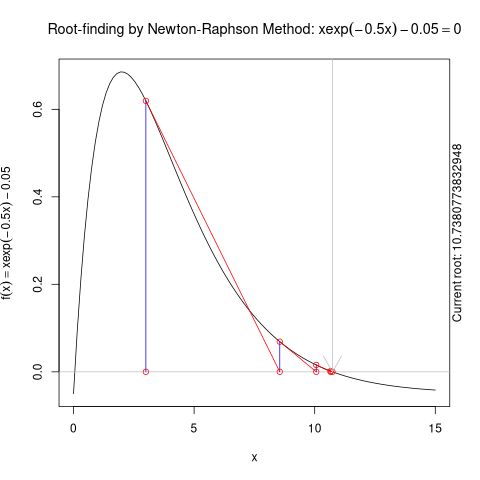
\includegraphics[width=.45\linewidth]{new-rap-2ex4}
%   \end{center}
%   %}
%   \pause

%   The algorithm terminates after 4 iterations. As an exercise, determine the first update, i.e. find $x_1$.
% \end{frame}

%\section{Gradient descent}
% \begin{frame}
%   \frametitle{Gradient descent}\pause
%   Given a differentiable convex function $f(x)$, 
%   \pause
%   two decisions must be made to reach its minimum point:\pause
%   \begin{itemize}[<+->]
%   \item \textit{direction} of descent
%   \item \textit{size} of step taken in that direction
%   \end{itemize}
%   \pause

  
%   \begin{block}{Steepest descent}\pause
%     The \textit{direction} of \textbf{\rd steepest descent} for $f(x)$ at a point $x_0$
%     is given by $\rd -\nabla f(x_0)$, \pause where $\nabla$ is the derivative operator. 
%   \end{block}
%   \pause
  
%   \bigskip
  
%   In gradient descent, we therefore use the update:\pause
%   \begin{equation}
%     \label{eq:15}\bl
%     x_{k+1} = x_k - \lambda f'(x_k)
%   \end{equation}
%   where $\gr \lambda>0$ is a small number called the \textbf{\gr learning rate}.
% \end{frame}


\section{Application: MLE}
\begin{frame}
  \frametitle{Maximum likelihood estimation: Key definitions}\pause
  Given a set of $n$ independent observations $x_1,x_2,\ldots,x_n$ from a random sample, the \textbf{likelihood function} is:
  \begin{equation}
    \label{eq:11}
    L(x_1,x_2,\ldots,x_n;\theta) \pause = f(x_1;\theta) \pause f(x_2;\theta) \pause \cdots \pause f(x_n;\theta)
  \end{equation}
  \pause
  The \textbf{maximum likelihood estimator (MLE)}, $\hat\theta$, \pause is the value of $\theta$ that maximizes the [log-]likelihood function:\pause
  \begin{equation}
    \label{eq:12}
    \pd{\ln L(x_1,x_2,\cdots,x_n;\theta)}{\theta} = \pause 0
  \end{equation}
  \pause
  For multiple parameters, the likelihood function is:\pause
  \begin{equation}
    \label{eq:13}
    L(x_1,\ldots,x_n;\theta_1,\ldots,\theta_1,\ldots,\theta_m) \pause = \prod_{i=1}^n f(x_i;\theta_i;\theta_1,\ldots,\theta_m)
  \end{equation}
  \pause
  And the MLE's would be found by simultaneously solving the partial derivatives set to 0 for each parameter.
\end{frame}

\begin{frame}
  \frametitle{Maximum likelihood estimation (MLE) in logistic
    regression}\pause

  The log-likelihood function for the binomial logistic regression case is \pause
  \begin{equation}
    \label{eq:16}
    \bl \ell(\beta) = \sum_i \lt[ y_i\lt(\beta_0 + \beta_1x_i \rt) - \log\lt(1 + e^{\beta_0 + \beta_1x_i}\rt) \rt]
  \end{equation}
  \pause
  The optimal $\hat{\beta}$ which maximizes $\ell(\beta)$ is the \textbf{\rd maximum likelihood estimate}.

  \pause

  \bigskip

  Also recall the derivative of $\ell$: \pause
  \begin{equation}
    \label{eq:17}
    \nabla_{\bm\beta}\ell = \pause
    \begin{pmatrix}
      {\pl \pd{\ell}{\beta_0}}\\[3mm]
      {\gr \pd{\ell}{\beta_1}}
    \end{pmatrix} = \pause
    \begin{pmatrix}
      \pl \sum_i \lt[y_i - p(x_i) \rt]\\[3mm]
      \gr \sum_i \lt[ x_i\lt(y_i - p(x_i)\rt)\rt] 
    \end{pmatrix}
  \end{equation}
  \pause
  We can use either Newton-Raphson or gradient \textit{\rd ascent} to \textit{\rd maximize} $\ell$.
\end{frame}

\begin{frame}
  \frametitle{Gradient ascent for MLE in logistic regression}
  \pause

  This approach only requires the first derivative:\pause
  \begin{equation}
    \label{eq:24}
    \beta_{k+1} = \beta_k + \lambda\nabla\ell(\beta_k)
  \end{equation}\pause
  Thus, to find $\hat\beta$ we iterate using:
  \pause
  \begin{equation}
    \label{eq:25}
    \begin{pmatrix}
      \beta_{0,k} \\ \beta_{1,k}
    \end{pmatrix}
    = \pause
    \begin{pmatrix}
      \beta_{0,k} \\ \beta_{1,k}
    \end{pmatrix}
    + \lambda
    \begin{pmatrix}
      \pl \sum_i \lt[y_i - p(x_i) \rt]\\[3mm]
      \gr \sum_i \lt[ x_i\lt(y_i - p(x_i)\rt)\rt] 
    \end{pmatrix}
  \end{equation}\pause
  
  Because the log-likelihood is \textit{\bl concave}, and thus a \textit{\bl maximization} problem,
  we \textit{\bl ascend} the function and thus
  \textit{\bl add} the scaled derivative.\pause

  
  \begin{itemize}[<+->]\rd
  \item As we can see, the gradient ascent method does not require a second derivative
  \item However, it may require more iterations to converge than Newton-Raphson
  \end{itemize}
  
\end{frame}

\begin{frame}
  \frametitle{Newton-Raphson approach for MLE in logistic regression}\pause
    The optimal point $\hat\beta$ is given by the root of the equation $\nabla_{\bm\beta}\ell = 0$.\pause

    \bigskip
    
    Applying Newton-Raphson, the update step is:\pause
    \begin{equation}
      \label{eq:nrupdate}
      \beta_{k+1} = \beta_k - {\bm H}^{-1}_{\beta_k}(\ell)\nabla_{\beta_k}\ell(\beta_k)
    \end{equation}
    \pause
    The operator $\bm H^{-1}$ represents the inverse \textbf{Hessian} (second derivative) matrix of $\ell$ with respect to
    $\beta$: \pause
    \begin{equation}
      \label{eq:19}
      {\bm H}_{\beta_k}(\beta_k) =\nabla_{\beta_k}^2\ell=
      \begin{pmatrix}
        \rd \pdd{\ell(\beta)}{\beta_0} & \pl \pd{^2\ell(\beta)}{\beta_0\beta_1} \\[2mm]
        \pl \pd{^2\ell(\beta)}{\beta_1\beta_0} &  \bl \pdd{\ell(\beta)}{\beta_1}\\
      \end{pmatrix}
    \end{equation}\pause
    Note that the \eqref{eq:nrupdate} is just the matrix representation of the 1-D case: \pause
    \begin{equation}
    \beta_{k+1} =\beta_k - \fr{\ell'(\beta_k)}{\ell''(\beta_k)}\label{eq:21}
  \end{equation}

\end{frame}

\begin{frame}
  \frametitle{Newton-Raphson approach for MLE (cont.)}\pause
  We can work out each component of the second derivative: \pause
  \begin{eqnarray}
    \label{eq:20}
    \rd \pdd{\ell(\beta)}{\beta_0} & \rd =& \rd - \sum_i p(x_i)(1 - p(x_i)) \\\pause
    \pl \pd{^2\ell(\beta)}{\beta_0\beta_1} & \pl =& \pl  - \sum_i x_i p(x_i)(1 - p(x_i)) \\\pause
    \bl \pdd{\ell(\beta)}{\beta_1} & \bl =& \bl  - \sum_ix_i^2 p(x_i)(1 - p(x_i)) 
  \end{eqnarray}
  \pause
  The complete update can then be shown as:\pause
  \begin{equation}
    \label{eq:22}
    \begin{pmatrix}
      \beta_{0,k+1}\\[3mm]
      \beta_{1,k+1}    
    \end{pmatrix}
     = 
    \begin{pmatrix}
      \beta_{0,k}\\[3mm]
      \beta_{1,k}
    \end{pmatrix}  -
    \lt[
    \begin{pmatrix}
      \rd \pdd{\ell(\beta)}{\beta_0} & \pl \pde{\ell(\beta)}{\beta_0}{\beta_1} \\[2mm]
      \pl \pde{\ell(\beta)}{\beta_1}{\beta_0} &  \bl \pdd{\ell(\beta)}{\beta_1}
    \end{pmatrix}^{-1}
    \begin{pmatrix}
      \pl \pd{\ell}{\beta_0}\\[2mm]
      \gr \pd{\ell}{\beta_1}
    \end{pmatrix}\rt]_{\beta_k}
  \end{equation}\pause
  Alternatively:\pause
  \begin{equation}
    \label{eq:28}
    \beta_{k+1}  = \beta_k - \lt[\lt(\pde{\ell(\beta)}{\beta}{\beta^T}\rt)^{-1} \pd{\ell(\beta)}{\beta}\rt]_{\beta_k}
  \end{equation}
\end{frame}

\section{Constrained optimization}

\begin{frame}
  \frametitle{Constrained optimization}
  \pe
  Deals with problems where we seek to minimize an objective:\pe
  \begin{equation}
    \min_{\bm\th\in\mc{C}}\mc{L}(\bm\th)
  \end{equation}\pe
  subject to:\pe
  \begin{align}
    h_i(\bm\th) &= 0, \quad i\in\mc{E}\\\pe
    g_j(\bm\th) &\le 0, \quad j\in\mc{I}
  \end{align}
  \pe
  where:
  \begin{itemize}
  \item $\mc{C}$: constraint/feasible set\pe
  \item $\mc{E}$: set of equality constraints \pe
  \item $\mc{I}$: set of inequality constraints
  \end{itemize}
\end{frame}


\begin{frame}
  \frametitle{Lagrange multipliers}
  \pe Given an optimization problem with $m$ equality contraints $\bm h(\bm\th)$, we can write the Lagrangian as:\pe
  \begin{equation}
    \mc L(\bm\th,\la) := \mc{L}(\bm\th) + \sum_{j=1}^m \la_jh_j(\bm\th)
  \end{equation}
  \pe
  where $\la_j$ are the Lagrange multipliers. \pe
  
  Thus, to find $\bm^*$, we solve:\pe
  \begin{equation}
    \nabla_{\bm\th,\la}L(\bm\th, \la) = \bm0
  \end{equation}
  \pe
  \begin{itemize}
  \item If $\bm\th \in \mb{R}^D$, there are $D+m$ equations with an equal number of unknonwns
  \end{itemize}
\end{frame}

\begin{frame}
  \frametitle{Karush-Kuhn-Tucker (KKT) conditions}
  \pe
  Given a problem with equality constraints $\bm h(\bm\th) = \bm 0$ and inequality constraints $\bm g(\bm\th) \le \bm 0$, the generalized Lagrangian is given by:\pe
  \begin{equation}
    \mc L(\bm\th,\bm\mu,\bm\la) = \mc{L}(\bm\th) +\pe \sum_i\mu_ig_i(\bm\th) + \sum_j\la_jh_j(\bm\th)
  \end{equation}\pe
  The optimization problem then becomes:
  \pe
  \begin{equation}
    \min_{\bm\th} \max_{\bm\mu\ge\bm 0,\bm\la}L(\bm\th,\bm\mu,\bm\la)
  \end{equation}
  \pe
  When $\mc{L}$ and $g$ are convex, then the KKT conditions are necessary and sufficient for global optimality: \pe
  \begin{itemize}
  \item Feasibility: constraints satisfied \pe
  \item Stationarity of solution: $\nabla_{\bm\th,\bm\mu,\bm\la}L = \bm0$\pe
  \item Dual feasibility: $\bm\mu \ge \bm0$\pe
  \item Complementary slackness: $\bm\mu \odot \bm g= \bm0$
  \end{itemize}
\end{frame}
\section{Outlook}


% \begin{frame}
%   \frametitle{Gradient descent}\pause

%   \begin{itemize}
%   \item Univariate case:\pause
%   \begin{equation}
%     \label{eq:15}\bl
%     x_{k+1} = x_k - \lambda f'(x_k)
%   \end{equation}
%   where $\gr \lambda>0$ is  the \textbf{\gr learning rate}.
%   \pause

%   \bigskip
% \item  Multivariate case: \pause
%   \begin{equation}
%     \bm x_{k+1} = \bm x_{k} - \lambda \nabla_{x}f(\bm x)
%   \end{equation}
% \end{itemize}

% \begin{alertblock}{Concave case}
%   If $f(x)$ is concave, then we maximize (gradient \textit{ascent}): \pause
%   \begin{equation}
%         x_{k+1} = x_k + \lambda f'(x_k)
%   \end{equation}
% \end{alertblock}
% \end{frame}



% \begin{frame}
%   \frametitle{Newton-Raphson for optimization}\pause
%   The Newton update for the root of a function $f(x)$ is given as:\pause
%     \begin{equation}
%       x_{k+1} = x_k - \fr{f(x_k)}{f'(x_k)}
%     \end{equation}
%     \pause
    
%     Given that the minimum of a convex function is at \pause $f'(x^{*}) = 0$, we solve this using Newton-Raphson (i.e.\
%     we find the root of $f'(x)$). \pause

%     \bigskip

%     \begin{block}{}
%       \begin{itemize}
%       \item Linearization:
%           \begin{equation}
%             \label{eq:12}
%             f'(x) \approx f'(x_0) + f''(x_0)(x - x_0) = 0
%           \end{equation}
%           \pause
%         \item Update:
%           \begin{equation}
%             x_{k+1} = x_k - \fr{f'(x_k)}{f''(x_k)}      
%           \end{equation}

%             \item Multivariate update: \pause
%     \begin{equation}
%       \bm x_{k+1} = \pause \bm x_{k} - \bm H_{\bm x_{k}}(f(x_{k}))^{-1}\nabla f(\bm x_{k})
%     \end{equation}
%         \end{itemize}
%     \end{block}

% \end{frame}

\begin{frame}
  \frametitle{Further topics}
  Some to be covered in Advanced Probabilistic ML:\pe
  \begin{itemize}
  \item Linear programming (simplex algorithm)
  \item Quadratic programming 
  \item Proximal gradient method
  \item Bound optimization (majorize-minimize algorithms)
  \item Expectation maximization (EM); for MLE/MAP estimation
    
  \end{itemize}
\end{frame}
\begin{frame}
  \frametitle{Reading assignments}

  \begin{itemize}
  \item \textbf{PMLI} 8
  \item \textbf{PMLCE} 5
  \end{itemize}
\end{frame}

% \begin{frame}
%   \frametitle{Introduction to Python/JupyterLab/R}
%   \pause

%   More will be said on this next lecture.

%   \pause

%   You can find a helpful tutorial at \url{https://cs231n.github.io/python-numpy-tutorial/#jupyter-and-colab-notebooks}.
% \end{frame}


\end{document}

%%% Local Variables:
%%% mode: latex
%%% TeX-master: t
%%% End:
